% Created 2019-05-28 Tue 22:01
% Intended LaTeX compiler: pdflatex
\documentclass{wx672ctexart}
\usepackage{wx672common}
\usepackage{wx672hyperref}
\usepackage{wx672minted}
\usepackage{wx672fonts}

\date{\textit{<2018-08-31 Fri>}}
\title{Shadowsocks in Debian}
\hypersetup{
 pdfauthor={},
 pdftitle={Shadowsocks in Debian},
 pdfkeywords={},
 pdfsubject={},
 pdfcreator={Emacs 25.2.2 (Org mode 9.1.13)}, 
 pdflang={Cn}}
\begin{document}

\maketitle
\tableofcontents


\section{基本工作原理图}
\label{sec:orgafd07c7}
\begin{center}
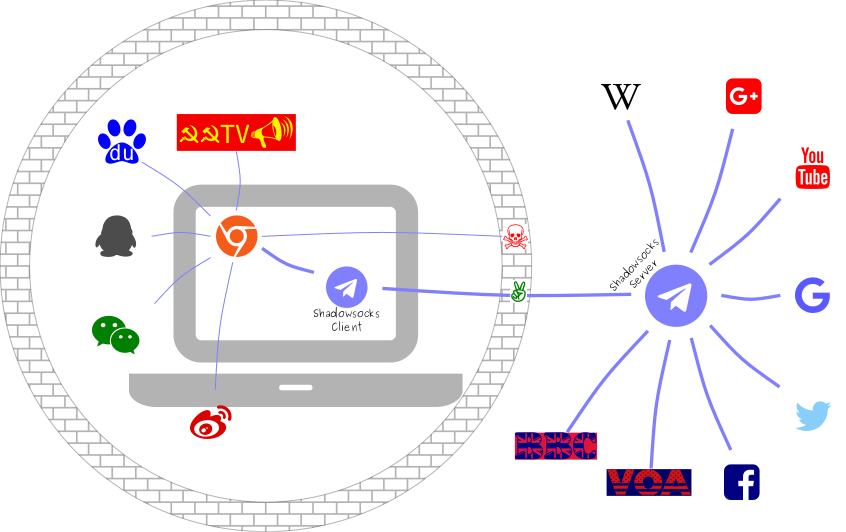
\includegraphics[width=.6\linewidth]{./ss.png}
\end{center}

要求:
\begin{enumerate}
\item 客户端:自行安装;
\item 服务器端:可以搜免费的;可以买现成的;也可以买墙外的云服务,自己安装服务器端;
\item 浏览器插件:自行安装。
\end{enumerate}

\section{客户端安装}
\label{sec:org3dc84e3}
\begin{verbatim}
sudo apt install shadowsocks-libev
\end{verbatim}
\section{客户端配置}
\label{sec:org4311b55}
Example: \texttt{/etc/shadowsocks-libev/config.json}

\begin{minted}[mathescape=true,linenos=true,numbersep=5pt,frame=lines,framesep=2mm]{javascript}
{
    "server":"127.0.0.1",
    "server_port":8388,
    "local_port":1080,
    "password":"fuPodNics",
    "timeout":60,
    "method":"chacha20-ietf-poly1305"
}
\end{minted}

简单注释:
\begin{enumerate}
\item 左花括号
\item 服务器的IP地址或域名;
\item 服务器端的端口号。本地客户端将向服务器的这个端口发起服务请求;
\item 客户端的端口号。本机的网络应用程序,比如浏览器,将向这个端口发起服务请求;
\item 客户端连接服务器端所需的密码;
\item 如果60秒还连不上服务器,就报错;
\item 加密方式;
\item 右花括号。
\end{enumerate}

补充说明:
\begin{enumerate}
\item 以上八行中的第2、3、5、7行信息都是由服务器端决定的。比如说,如果你是花钱买的现成服务,那么实际上你花钱买的(除了流量)就是这几条信息。第4行,客户端的端口号,默认都是1080,可以自己改,但通常没必要;
\item 如果是买的现成服务,那么通常服务器的数量不止一个。你应该为每个服务器都单写一个配置文件。
这样如果一个服务器连不上了,你可以迅速切换到另一个。比如说,你原来用的是
\texttt{/etc/shadowsocks-libev/a.json}:
\begin{verbatim}
ss-local -v -c /etc/shadowsocks-libev/a.json
\end{verbatim}

后来忽然连不上了,那么你可以按 \texttt{Ctrl-c} 终止这个进程。然后再另起一个:
\begin{verbatim}
ss-local -v -c /etc/shadowsocks-libev/b.json
\end{verbatim}
\item 把你的所有配置文件都放在一个目录里,通常是 \texttt{/etc/shadowsocks-libev/} 。
\end{enumerate}

\section{Chrome浏览器插件的安装配置}
\label{sec:org1d21325}
插件的作用是让你的浏览器“该翻墙的时候翻墙,不该翻墙的时候就不翻墙”,所以严格讲,它不是必需的。在没有插件的情况下,使用下面这两条命令你就已经可以翻墙了:
\begin{verbatim}
ss-local -v -c /etc/shadowsocks-libev/b.json
google-chrome --proxy-server='socks5://127.0.0.1:1080'
\end{verbatim}


Chrome浏览器的插件通常只能从\href{https://chrome.google.com/webstore/category/extensions?utm\_source=chrome-ntp-icon}{Chrome Web Store}安装。很不幸,访问这个网站就要先能翻墙才行。办法就是利用上面两条命令。在命令行执行这条命令之后,如果网断了,而且看到较多的出错信息,比如:
\begin{verbatim}
2018-08-31 19:37:50 ERROR: server_recv_cb_recv: Connection reset by peer
2018-08-31 19:37:50 ERROR: server_recv_cb_recv: Connection reset by peer
2018-08-31 19:37:50 ERROR: server_recv_cb_recv: Connection reset by peer
2018-08-31 19:37:50 ERROR: server_recv_cb_recv: Connection reset by peer
2018-08-31 19:37:50 ERROR: server_recv_cb_recv: Connection reset by peer
\end{verbatim}
那么,就换c.json、d.json……试试。

\begin{enumerate}
\item 安装插件Switchy Omega
\begin{itemize}
\item \url{https://chrome.google.com/webstore/detail/proxy-switchyomega/padekgcemlokbadohgkifijomclgjgif?utm\_source=chrome-ntp-icon}
\end{itemize}
\item 如果上面三步都顺利完成了,那么现在可以关掉浏览器了,然后重新打开它,但不要添加代理选项:
\begin{verbatim}
google-chrome
\end{verbatim}
\item 配置插件在浏览器窗口的右上角找到Switchy Omega的图标,然后配置吧。

\begin{center}
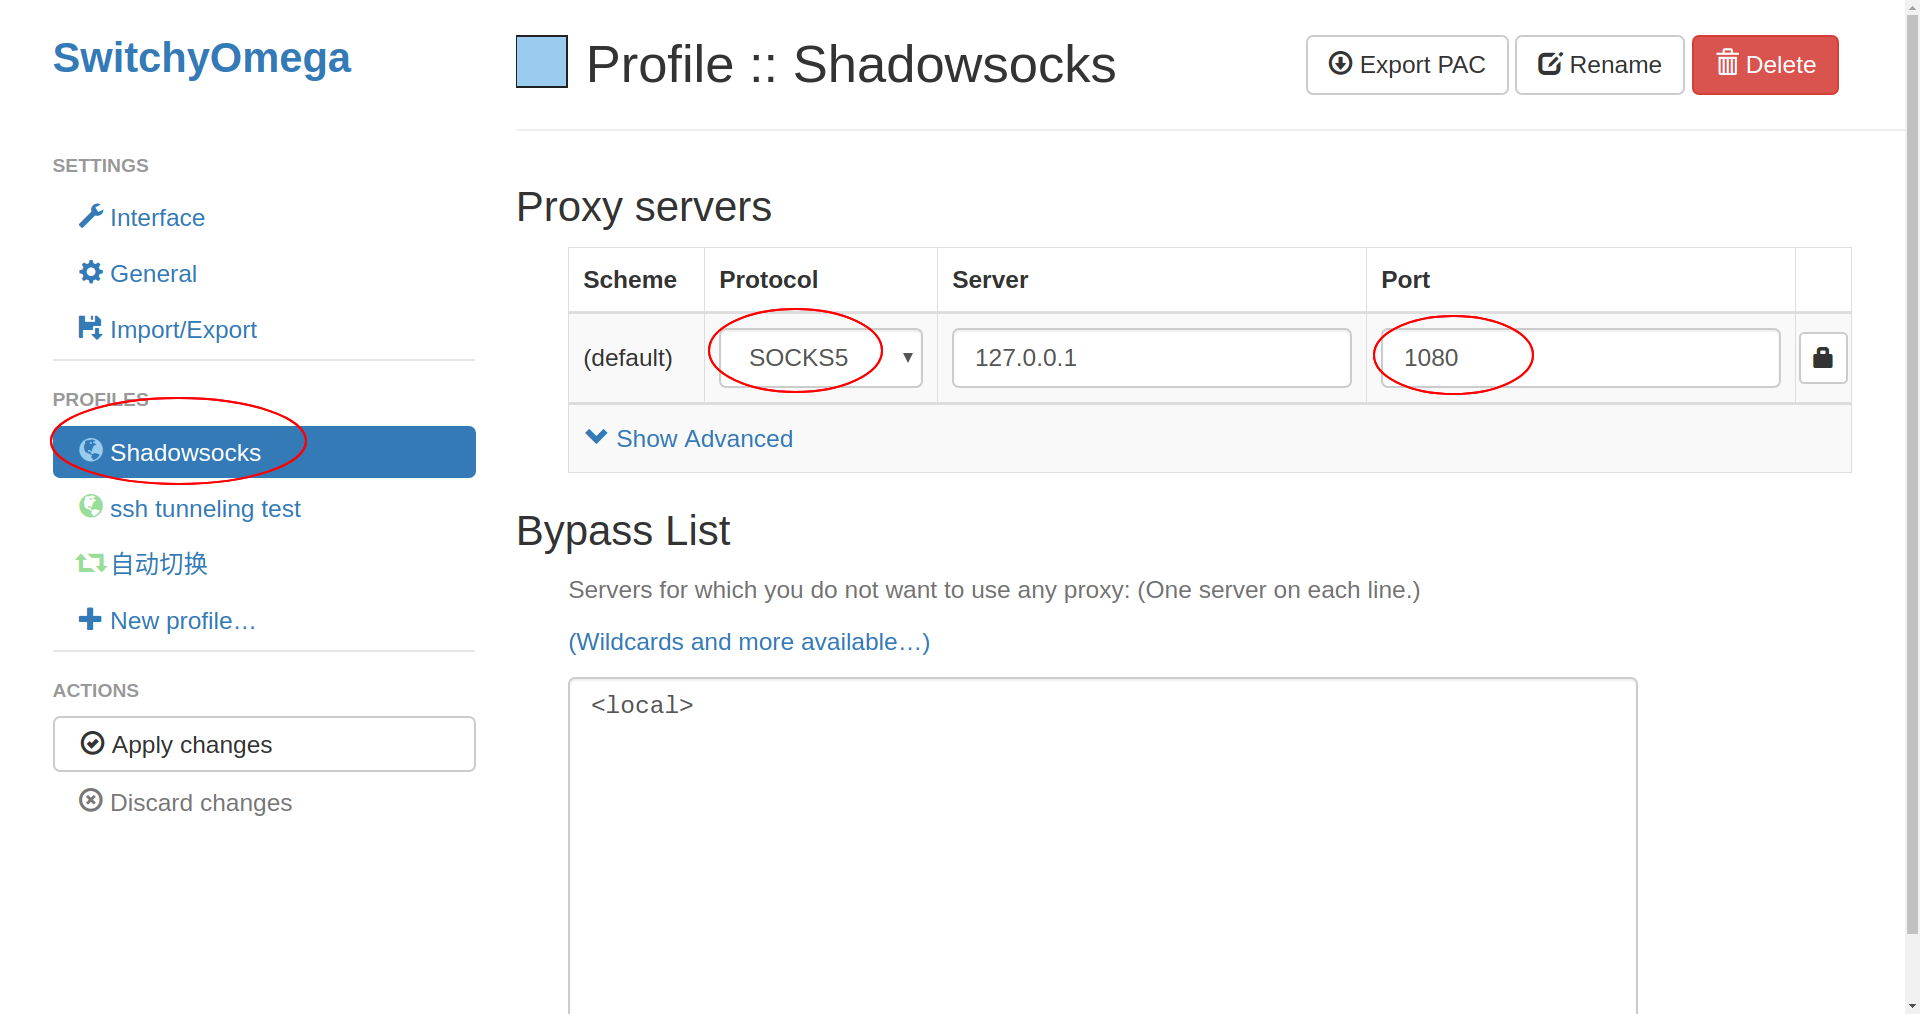
\includegraphics[width=.6\linewidth]{./switchyomega1.png}
\end{center}

如果你想让插件来判断什么时候该翻墙的话,就需要预先给它输入一系列的规则,这显然是很累人的。所以,通常是去网上搜到人家\href{https://github.com/shminer/SwitchyOmega-backup}{现成的配置},然后把它import进来就行了。
\end{enumerate}

简单总结一下要点:
\begin{enumerate}
\item 要先启动本地代理:
\begin{verbatim}
ss-local -v -c /etc/shadowsocks-libev/b.json
\end{verbatim}
\item 要把浏览器插件配置好。
\end{enumerate}
\end{document}
%%% Local Variables:
%%% mode: latex
%%% TeX-master: t
%%% End:
